\chapter{Scaling and Accuracy of atomic-orbital based SOS-ADC(2)}

The theoretical groundwork for CD-DF-SOS-ADC(2) was laid out in detail in the previous chapters. In this chapter, the performance of the method is explored in terms of scaling, memory footprint and accuracy. First, the J, K and Z kernels are analyzed in the context of ground state Hartree-Fock and SOS-MP2 calculations. They form the heart of the AO-SOS-ADC(2) machinery and a separate analysis is therefore justified. Moreover, bugs and performance issues are easier to spot. In the second part of this chapter, the performance of the AO-SOS-ADC(2) method itself is investigated. Results are then summarized at the end of this chapter. 

\section{Computational Details}

If not stated otherwise, results presented in this chapter were obtained using MEGALOchem, an open-source quantum chemistry package which provides an optimized environment for algorithms exploiting the sparsity of the AO basis. For more details, the reader is referred to the subsequent chapters.

Reference values for Hartree-Fock and SOS-MP2 energies, as well as excitation energies for canonical SOS-ADC(2) were obtained with version 5.1 of the Q-Chem quantum chemistry package.

All calculations that use MEGALOchem have been performed on two nodes with two Intel E5-2690v3 Haswell CPUs and 512 GB RAM each (48 cores in total), located on the Tegner cluster at the PDC in Stockholm. Absolute wall times for scalings should not be considered, as developmental builds of MEGALOchem are used, and MPI processes are not optimally distributed.  

\section{Ground-state Prerequisites}

\subsection{Molecular Test Systems}

Virtually all works that present some form of low-scaling electronic structure methods use linear alkanes (LA) as their test systems. Linear molecular system represent a best case scenario where the overlap between basis functions $\mu$, $\nu$ decays very rapidly as function of distance $r_{\mu\nu}$. The low scaling regime can generally be reached quite quickly, which is great for getting a first impression on the performance on the methods. Unfortunately, linear systems like alkanes are chemically uninteresting. For this reason, the present benchmarking also looks at the worst case scenario of spherically shaped and thus electron-dense molecular system, in this case hydrated formamide (FW) with differently sized solvation shells. For systems such as these, the strength of electron correlation effects decreases much more slowly as a function of increasing system size $N$. The systems are illustrated in Figure \ref{fig:GS_MOL}. LA structure are taken from \ref{Och2021} and FW structures from \ref{Bau2017}.

Basis sets also play an important role. For correlated methods such as MP2, Coupled Cluster and their excited state analogs, triple-zeta quality basis sets are mandatory for obtaining accurate results for small to medium-sized molecules. A larger basis set implicates a larger virtual space to capture correlation effects. Fortunately, for larger molecules, basis set superposition makes larger basis sets less crucial. Here, the small but still routinely used cc-pVDZ basis set is considered for the computation of ground state properties. For Hartree-Fock and MP2, the auxiliary basis sets cc-pVDZ-jkfit and cc-pVDZ-ri are used, respectively.

Table \ref{tab:GS_NBAS} shows the total number of basis functions of the systems considered in this section. The length of the alkane chains and the size of the solvation shell of FW are chosen such that they are on the same order of magnitude. For each system type, four sizes are chosen.

\begin{figure}
     \centering
     \begin{subfigure}{0.4\textwidth}
         \centering
         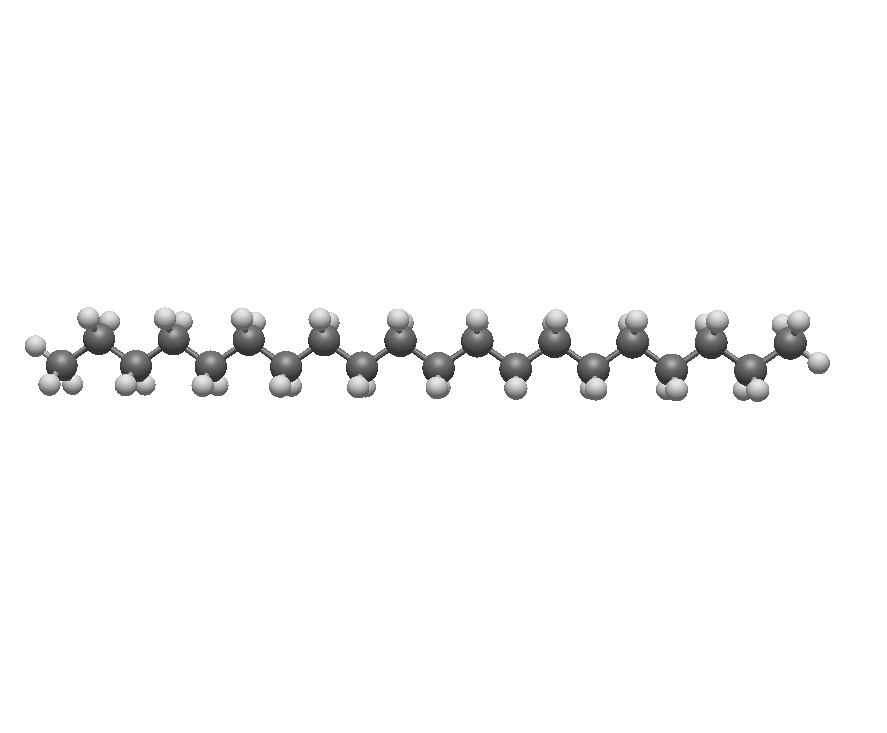
\includegraphics[width=\textwidth]{Pics/alkan.png}
         \caption{}
     \end{subfigure}
	\begin{subfigure}{0.5\textwidth}
         \centering
         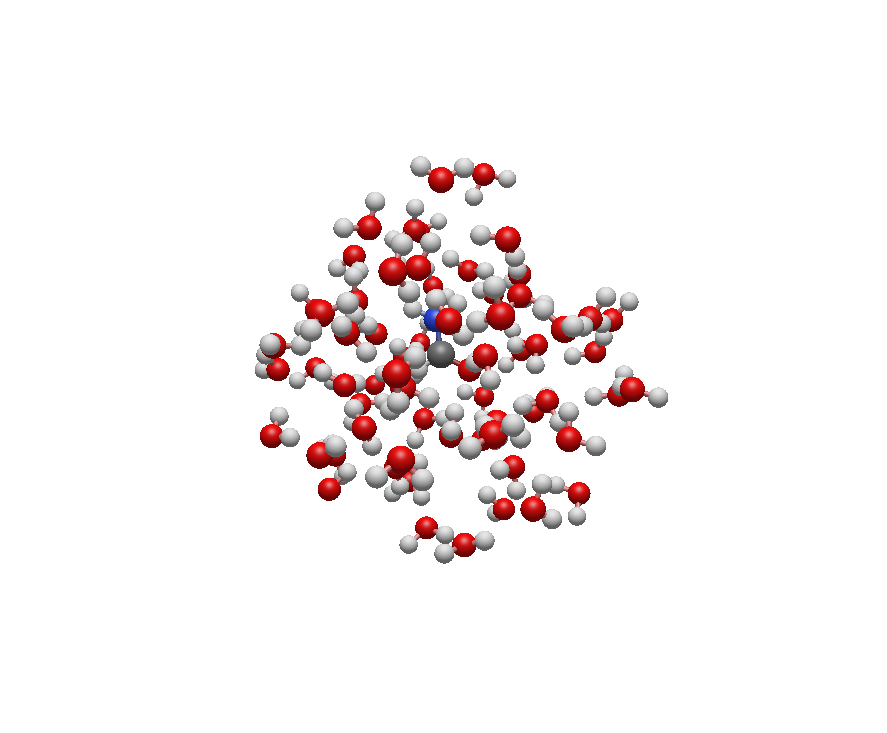
\includegraphics[width=\textwidth]{Pics/FW63.png}
         \caption{}
         \label{fig:five over x}
     \end{subfigure}
     	\caption{Molecular systems used for the analysis of the J, K and Z kernels: (a) linear alkanes (LA); (b) hydrated formamide (FW)}
        \label{fig:GS_MOL}
\end{figure}

\begin{table}
\centering
\begin{tabular}{llllll}
\hline
\multicolumn{3}{c}{LA} & \multicolumn{3}{c}{FW} \\ \hline
Molecule & Abbrev. & $N_{AO}$ & Molecule & Abbrev. $N_{AO}$ \\ \hline
H$_{42}$C$_{20}$ & LA20 & 490 & H$_{33}$CNO$_{16}$ & FW15 & 417 \\
H$_{82}$C$_{40}$ & LA40 & 970 & H$_{63}$CNO$_{31}$ & FW30 & 777 \\
H$_{162}$C$_{80}$ & LA80 & 1930 & H$_{129}$CNO$_{64}$ & FW63 & 1569  \\
H$_{322}$C$_{160}$ & LA160 & 3850 & H$_{291}$CNO$_{145}$ & FW144 & 3513 \\
\hline  
\end{tabular}
\label{fig:GS_NBAS}
\caption{Molecular formula for the considered systems and the number of basis functions for cc-pVDZ}
\end{table}

\subsection{Illustrating the Scaling}

There are generally two ways how scaling is illustrated in literature: (1) a graph that shows the total wall time as a function of increasing system size and/or (2) a table with scaling coefficients computed relative to a previous system size as
\begin{equation}
x = \frac{log(N_i/N_{i-1})}{log(T_i/T_{i-1})}
\end{equation} 
\noindent Graphs are most useful to show the prefactor of the methods, while tables are much better suited for showing the polynomial scaling, as the differences between e.g. $\ccpx{2}$ and $\ccpx{2.5}$ are difficult to pick up with the naked eye. Here, both methods are used. 

\FloatBarrier

\subsection{Integral Evaluation}

The J and K kernels have the tensors $B_{X\mu\nu}$ and $M_{XY}$ as common input. They are defined by
\begin{equation}
\cn{\mu\nu}{\lambda\sigma} = B_{X\mu\nu} M_{XY} B_{X\lambda\sigma}
\end{equation}
\noindent Three different density fitting approximations are considered for benchmarking: the standard density fitting in the coulomb metric (DFCM), local density fitting in the coulomb attenuated metric with the complimentary error function (DFCAM), and quasi-robust density fitting (QRDF). The exact form of $\mbf{B}$ and $\mbf{M}$ depends on the DF approximation (Table \ref{tab:BMTENSORS}). If not indicated otherwise, DFCAM uses an attenuation factor of 0.1, and QRDF uses $T$ = 1e-5 and $R$ = 40. 

\begin{table}
\centering
\begin{tabular}{lcc}
\hline
DF method & $B^X_{\mu\nu}$ & $M_{XY}$ \\
\hline
DFCM & $\cn{X}{\mu\nu}$ &  $\cn{X}{Y}^{-1}$ \\
DFCAM & $\cn{X}{\mu\nu}_{\omega}$ & $\cn{X}{Y}_{\omega}^{-1} \cn{Y}{R} \cn{R}{S}_{\omega}^{-1}$ \\
QRDF & $C^{QRDF}_{X\mu\nu}$ & $\cn{X}{Y}$ \\ 
\hline
\end{tabular}
\label{tab:BMTENSORS}
\caption{Expressions for $\mbf{B}$ and $\mbf{M}$ for kernels presented in this work. The subscript $\omega$ indicates that the coulomb attenuated metric is used.}
\end{table}

Figure \ref{fig:GS_BTIME_ALKAN} shows the time needed to evaluate $\mbf{B}$ for the LA systems. There is no difference between DFCM and DFCAM, hence only DFCM is shown. QRDF has a much higher prefactor due to the huge number of QR decompositions that are necessary for the calculation of the fitting coefficients. The consequence is that QRDF is an order of magnitude more expensive than DFCM or DFCAM. Comparing the wall times here to the the total time needed for the Hartree-Fock procedure, QRDF is actually more expensive than the hole HF computation for LA20, LA40 and LA80. However, QRDF has the advantage of becoming linearly scaling going from LA80 to LA160, compared to the quadratic scaling of DFCM.  

In QRDF, the test functions $\{Q\}$ for the fitting procedure are chosen based on overlap criteria with the fitting functions $\{P\}$ (Equation \ref{eq:QRDF_TEST}). Here lies the reason for the massive overhead of QRDF: in the original implementation by Tew, the smallest exponent of a GTO is chosen for determining the overlap between $\mu_Q$ and $\nu_P$. In the QRDF procedure as implemented in MEGALOchem, the scheme is generalized to \emph{blocks} of basis shells centered on the same atom, i.e. the smallest exponent of the whole block is used for the overlap screening. This had the unwanted side-effect that the screening for the test functions is much harsher than necessary. Even if the overlap values for most exponents of a block with another block are zero, only one exponent decides whether the block is included in the fitting procedure. A more lenient criteria based on an average overlap or matrix norm can reduce the overhead with little impact on accuracy. For the remainder of this chapter, the original, strict version of the QRDF algorithm is used. A newer version of the QRDF procedure is currently being developed. The strictness of the method has no impact on the sparsity of the fitting coefficients, and hence all findings on the scaling of the kernels will still be valid for the new implementation.

Figure \ref{fig:GS_BNZE_ALKAN} shows the number of non-zero elements of $\mbf{B}$ for LA. Quadratic scaling can be observed for DFCM, and linear scaling for DFCAM and QRDF. An interesting observation is that $\mbf{B}$ is evaluated with $\ccpx{2}$ effort in DFCAM, but it scales linearly in its elements. This is due to the screening procedure: for DFCAM, the normal DFCM Schwarz screening is used, which does not take into account the exponential decay between $\cbra{X}$ and $\cket{\mu\nu}$. More strict screening procedures could be introduced to speed up integral evaluation of DFCAM, which will be especially useful for direct algorithms. Similarly, the QRDF scheme has mostly cubic scaling effort for evaluation, but ultimately the elements scale linearly with system size. 

Finally, Figure \ref{fig:GS_BNZE_FW} shows the memory footprint of $\mbf{B}$ for the hydrated formamide systems. The tensors are naturally much more dense due to the molecular structure. Nonetheless, the QRDF fitting coefficients still scale quite favorably. Unfortunately, the QRDF procedure itself takes ten times longer than the HF calculation itself. Whether this is due to the strictness of QRDF, or just the nature of QRDF itself, is a point for further investigation. For now, QRDF is not considered useful for dense electronic systems. 

To compute $\mbf{M}$ in DFCM and DFCAM, a matrix inversion needs to computed, which scales with $\ccpx{3}$. For the system sizes considered in this report, the relative wall times for matrix inversions are small compared to all other steps. The QR decompositions in QRDF also scale cubically, although the size of the linear lest squares problem will eventually become constant, i.e. the number of test functions will be independent of system sizes. This is a major advantage of QRDF, although as was already pointed out, it does matter for the current molecular sizes.

%%%%%%%%%%%%%%%%%%% MEMORY INTEGRALS (LA) %%%%%%%%%%%%%%%%%%%%%%%
\begin{figure}
\begin{minipage}[t]{0.5\textwidth}
\vspace{0pt}
\centering
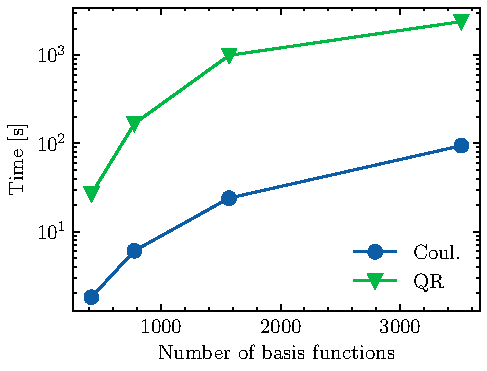
\includegraphics[width=\textwidth]{../articles/art1/qrtime_alkan}
%\captionof{figure}[This Figure]{Figure}
%\par
\end{minipage}
\begin{minipage}{0.4\textwidth}
\vspace{0pt}
\centering
\begin{tabular}{rrr}
\hline
N$_{AO}$ & DFCM & QRDF \\ \hline
490 & --- & --- \\ 
970 & 1.94 & 2.95 \\ 
1930 & 1.96 & 2.53 \\ 
3850 & 1.70 & 1.09 \\ \hline
\end{tabular}
%\captionof{table}[This Table]{Table}
%\par\vspace{0pt}
\end{minipage}
\caption{Total walltime needed to construct the tensor $B_{X\mu\nu}$ (3c2e integrals, QR fitting coefficients) for LA}
\label{fig:GS_BTIME_ALKAN}
\end{figure}
%
%
\begin{figure}
\begin{minipage}{0.5\textwidth}
\centering
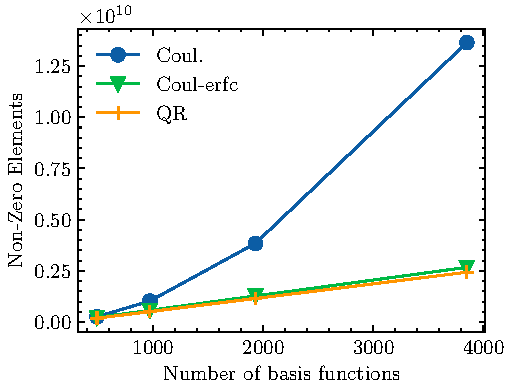
\includegraphics[width=\textwidth]{../articles/art1/eri_nze_alkan}
\end{minipage}
%\hspace{0.05\textwidth}
\begin{minipage}{0.4\textwidth}
\centering
\begin{tabular}{rrrr}
\hline
N$_{AO}$ & DFCM & DFCAM & QRDF \\ \hline
490 & --- & --- & --- \\ 
970 & 2.01 & 1.37 & 1.45 \\ 
1930 & 1.92 & 1.16 & 1.18 \\ 
3850 & 1.83 & 1.07 & 1.08 \\ \hline
\end{tabular}
\end{minipage}
\caption{Number of non-zero elements in the tensor $B_{X\mu\nu}$ as a function of $N_{AO}$ for LA, with the corresponding scaling coefficients}
\label{fig:GS_BNZE_ALKAN}
\end{figure}
%
%
\begin{figure}
\begin{minipage}{0.5\textwidth}
\centering
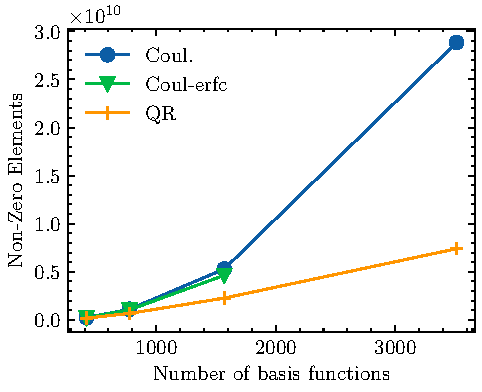
\includegraphics[width=\textwidth]{../articles/art1/eri_nze_fw}
%\captionof{figure}[This Figure]{Figure}
\end{minipage}
\begin{minipage}{0.4\textwidth}
\centering
\begin{tabular}{rrrr}
\hline
N$_{AO}$ & DFCM & DFCAM & QRDF \\ \hline
417 & --- & --- & --- \\ 
777 & 2.50 & 2.45 & 2.15 \\ 
1569 & 2.23 & 2.11 & 1.73 \\ 
3513 & 2.10 & --- & 1.47 \\ \hline
\end{tabular}
%\captionof{table}[This Table]{Table}
\end{minipage}
\caption{Number of non-zero elements in the tensor $B_{X\mu\nu}$ as a function of $N_{AO}$ for FW, with the corresponding scaling coefficients}
\label{fig:GS_BNZE_FW}
\end{figure}

\subsection{Hartree-Fock}

\subsubsection{Scaling: Coulomb Matrix}

The coulomb matrix is evaluated as
\begin{align}
d_X = M_{XY} B_{Y\mu\nu} P_{\nu\mu} \\
J_{\mu\nu} = B_{X\mu\nu} d_X
\end{align}
\noindent The scaling of the individual steps is not considered, but only the total time needed to construct the coulomb matrix. Figure \ref{fig:GS_DFJSCALE_LA} shows the scaling behavior of the J kernel for the LA systems. DFCM does not lower the scaling compared to the exact evaluation of the coulomb matrix which scales quadratically if sparse matrix algebra is used. Local metrics can however lower the scaling by an order of magnitude. QRDF even exhibits sublinear scaling from LA80 to LA160. The sublinear scaling originates from the increased sparsity of $\mbf{M}$. While DFCM and DFCAM need to invert matrices, which also destroys sparsity, QRDF only needs the 2c2e integrals which have an $1/R^{l+1}$ decay between centers. Although this decay is slow, it is faster compared to the 4c2e integrals and can affect the scaling positively.

Table \ref{tab:GS_DFJKSCALE_FW} shows the scaling coefficients for the FW systems. Here, DFCAM and QRDF do not give any considerable advantage over DFCM. %(ABSOLUTE???)

\subsubsection{Scaling: Exchange Matrix}

The exchange matrix is computed as
\begin{align}
C_{X\mu\nu} &= M_{XY} B_{Y\mu\nu} \\
K_{\mu\nu} = B_{X\nu\sigma} C_{X\mu\lambda} P_{\lambda\sigma} 
\end{align}
\noindent Both steps are analyzed separately. Step 1 actually only needs to be evaluated once, while step 2 is repeated at each iteration. Figure \ref{fig:GS_DFK1SCALE_LA} illustrates the scaling for step 1 for linear alkanes. It is the most expensive step of the Hartree-Fock procedure in terms of scaling (ignoring diagonalization and matrix inversion), and profits most from the local density fitting approximation. The computational effort can be reduced to $\ccpx{2}$ and almost $\mathcal{O}(N)$ for QRDF. Step 1 forms a 3-index tensor which needs to be stored in memory. The sparsity of this tensor is illustrated in Figure \ref{fig:GS_MBNZE_LA}. The number of elements scales approximately quadratically for all metrics, although QRDF has a slight edge on the other methods. It appears that local density fitting approximations do not have a lot of impact on the memory requirements of step 1, although they can speed up the computation considerably. 

Step 2 is less expensive, but still more demanding than the computation of the coulomb matrix. Figure \ref{fig:GS_DFK2SCALE_LA} shows the scaling for linear alkanes. Moreover, the MO algorithm is also included for comparison. Even standard density fitting can positively impact the scaling, with a reduction from cubic to $\ccpx{1.5}$. DFCAM does not improve on the scaling, although the additional sparsity lowers the prefactor compared to DFCM. QRDF can again achieve linear scaling, for similar reasons as discussed above. 

Finally, the scaling coefficients for the FW systems are collected in Table \ref{tab:GS_DFJKSCALE_FW}. As expected, local density fitting does not considerably reduce the scaling for evaluating the exchange matrix and shows the limit of what AO methods can do. Of course, at some point, the computational effort will eventually decrease with increasing system size $N$, although the crossover point is much later than for LA. The major advantage is that, compared to a MO implementation, local density fitting decreases the overhead compared to DFCM, making it more competitive to the MO methods (Figure \ref{fig:GS_DFK2SCALE_FW}). The AO method is therefore still applicable in a dense context. 

For FW, numerical issues were encountered for FW144, hence this point is missing in the tables and figures.

%%%%%%%%%%%%%%%%% SCALING (LA) %%%%%%%%%%%%%%%%%%%%
\begin{figure}
\begin{minipage}{0.5\textwidth}
\centering
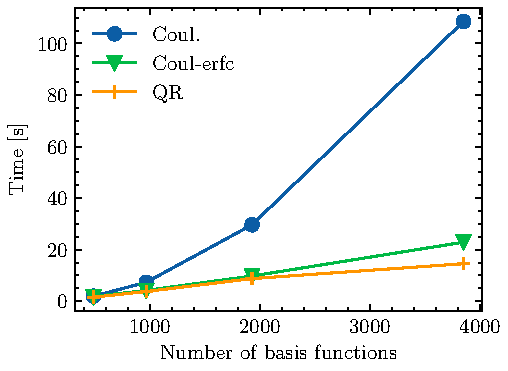
\includegraphics[width=\textwidth]{../articles/art1/hfJ_alkan}
%\label{fig:GS_DFJSCALE_LA}
%\captionof{figure}{Average wall time for constructing the coulomb matrix as a funtion of $N_{AO}$ (LA)}
\end{minipage}
%\hspace{0.05\textwidth}
\begin{minipage}{0.4\textwidth}
\centering
\begin{tabular}{rrrr}
\hline
N$_{AO}$ & DFCM & DFCAM & QRDF \\ \hline
490 & --- & --- & --- \\ 
970 & 1.93 & 1.23 & 1.29 \\ 
1930 & 2.03 & 1.23 & 1.23 \\ 
3850 & 1.88 & 1.23 & 0.73 \\ \hline
\end{tabular}
%\label{tab:GS_DFJSCALE_LA}
%\captionof{table}{Scaling factors for contruction of the coulomb matrix (LA)}
\end{minipage}
\caption{Scaling behaviour for the construction of the coulomb matrix using different metrics (LA)}
\label{fig:GS_DFJSCALE_LA}
\end{figure}
%
\begin{figure}
\begin{minipage}{0.5\textwidth}
\centering
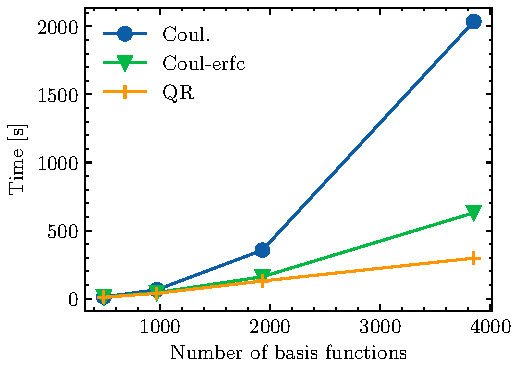
\includegraphics[width=\textwidth]{../articles/art1/hfK1_alkan}
%\captionof{figure}[Scaling of K kernel (step 1) for linear alkanes]{Average wall time for constructing the exchange matrix (step 1: $M_{XY}B_{Y\mu\nu}$ ) as a funtion of $N_{AO}$ (LA)}
%\label{fig:GS_DFK1SCALE_LA}
\end{minipage}
%\hspace{0.05\textwidth}
\begin{minipage}{0.4\textwidth}
\centering
\begin{tabular}{rrrr}
\hline
N$_{AO}$ & DFCM & DFCAM & QRDF \\ \hline
490 & --- & --- & --- \\ 
970 & 2.43 & 1.97 & 1.96 \\ 
1930 & 2.49 & 1.89 & 1.78 \\ 
3850 & 2.53 & 1.98 & 1.21 \\ \hline
\end{tabular}
%\captionof{table}{Scaling factors for contruction of the exchange matrix, step 1 (LA)}
%\label{tab:GS_DFK1SCALE_LA}
\end{minipage}
\caption{Scaling behaviour for the construction of the exchange matrix (step1) using different metrics (LA)}
\label{fig:GS_DFK1SCALE_LA}
\end{figure}
%
\begin{figure}
\begin{minipage}{0.5\textwidth}
\centering
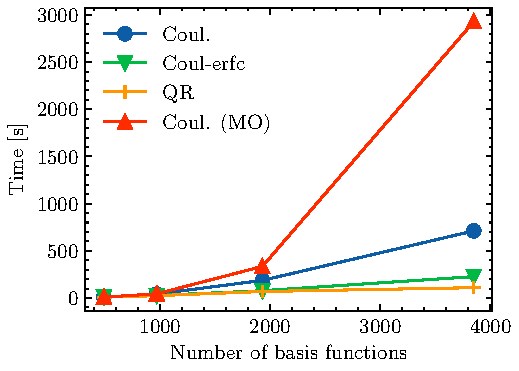
\includegraphics[width=\textwidth]{../articles/art1/hfK2_alkan}
%\captionof{figure}[Scaling of K kernel (step 2) for linear alkanes]{Average wall time for constructing the exchange matrix (step 2: $B_{X\nu\lambda} C_{X\mu\sigma} P_{\sigma\lambda}$) as a funtion of $N_{AO}$ (LA)}
%\label{fig:GS_DFK2SCALE_LA}
\end{minipage}
%\hspace{0.05\textwidth}
\begin{minipage}{0.3\textwidth}
\centering
\begin{tabular}{rrrrr}
\hline
N$_{AO}$ & DFCM & DFCAM & QRDF & DFMO \\ \hline
490 & --- & --- & --- & --- \\ 
970 & 1.58 & 1.58 & 1.60 & 2.34 \\ 
1930 & 1.57 & 1.57 & 1.50 & 2.96 \\ 
3850 & 1.56 & 1.56 & 0.67 & 3.14 \\ \hline
\end{tabular}
%\captionof{table}{Scaling factors for contruction of the exchange matrix, step 2 (LA)}
%\label{tab:GS_DFK2SCALE_LA}
\end{minipage}
\caption{Scaling behaviour for the construction of the exchange matrix (step 2) using different metrics (LA)}
\label{fig:GS_DFK2SCALE_LA}
\end{figure}

%%%%%%%%%%%%%%%%% SCALING (FW) %%%%%%%%%%%%%%%%%%%%%%%

\begin{table}
\footnotesize
\begin{tabular}{r|rrr|rrr|rrrr}
\hline
 & \multicolumn{3}{c}{J} & \multicolumn{3}{c}{K (STEP 1)} &   \multicolumn{4}{c}{K (STEP 2)} \\ \hline
N$_{AO}$ & DFCM & DFCAM & QRDF & DFCM & DFCAM & QRDF & DFCM & DFCAM & QRDF & DFMO \\ \hline
417 & --- & --- & --- & --- & --- & --- & --- & --- & --- & --- \\ 
777 & 2.18 & 2.20 & 1.88 & 2.77 & 2.77 & 2.51 & 2.55 & 2.55 & 2.33 & 2.33 \\ 
1569 & 2.32 & 1.71 & 1.28 & 2.77 & 2.18 & 1.85 & 2.82 & 2.13 & 1.67 & 2.86 \\ 
3513 & 2.08 & --- & 1.94 & 2.79 & --- & 2.74 & 2.59 & --- & 2.65 & 3.13 \\ \hline
\end{tabular}
\caption{Scaling coefficients for the J kernel and the two steps of the K kernel (FW)}
\label{tab:GS_DFJKSCALE_FW}
\end{table}

\begin{figure}
\centering
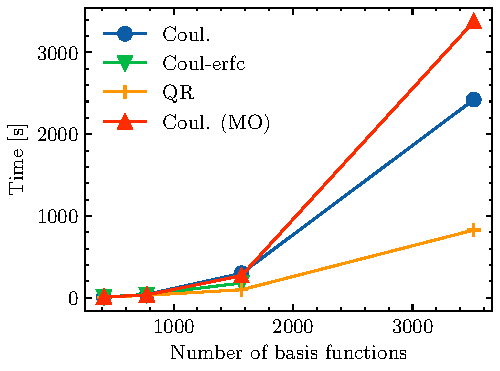
\includegraphics[scale=1.0]{../articles/art1/hfK2_fw}
\label{fig:GS_DFK2SCALE_FW}
\caption{Scaling for the construction of the exchange matrix (step 2) for hydrated formamide. Although local density approximations do not lower the scaling, a reduction of the prefactor can be observed.}
\end{figure}

%%%%%%%%%%%%%%%%% MEMORY (LA/FW) %%%%%%%%%%%%%%%%%%%%%%%%

%
\begin{figure}
\begin{minipage}{0.5\textwidth}
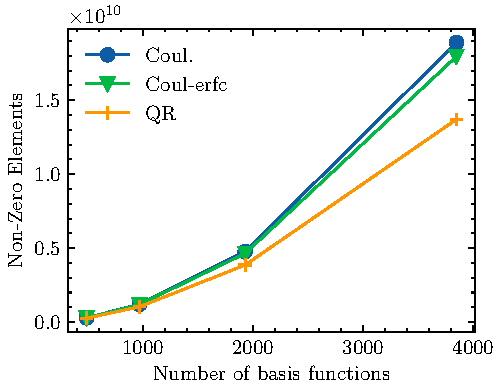
\includegraphics[width=\textwidth]{../articles/art1/cfit_nze_alkan}
%\captionof{figure}{Number of non-zero elements of $M_{XY}B_{Y\mu\nu}$ as a function of $N_{AO}$ (LA)}
\end{minipage}
%\hspace{0.05\textwidth}
\begin{minipage}{0.3\textwidth}
\begin{tabular}{rrrr}
\hline
N$_{AO}$ & DFCM & DFCAM & QRDF \\ \hline
490 & --- & --- & --- \\ 
970 & 2.07 & 2.06 & 2.01 \\ 
1930 & 2.01 & 1.98 & 1.92 \\ 
3850 & 1.99 & 1.96 & 1.84 \\ \hline
\end{tabular}
%\captionof{table}{Scaling coefficients of $M_{XY}B_{Y\mu\nu}$ (LA)}
\end{minipage}
\caption{Number of non-zero elements of the tensor $M_{XY}B_{Y\mu\nu}$ as a function of $N_{AO}$ }
\label{fig:GS_MBNZE_LA}
\end{figure}
%
\begin{figure*}
\begin{minipage}{0.5\textwidth}
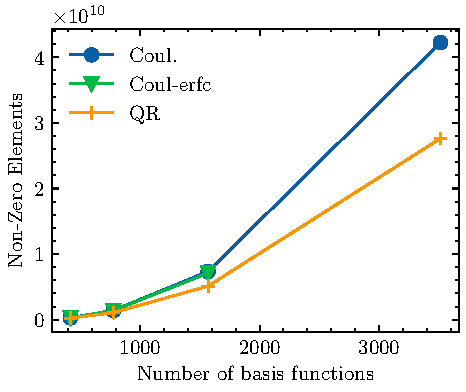
\includegraphics[width=\textwidth]{../articles/art1/cfit_nze_fw}
\captionof{figure}{Number of non-zero elements of $M_{XY}B_{Y\mu\nu}$ as a function of $N_{AO}$ (FW)}
\end{minipage}
\hspace{0.05\textwidth}
\begin{minipage}{0.3\textwidth}
\begin{tabular}{rrrr}
\hline
N$_{AO}$ & DFCM & DFCAM & QRDF \\ \hline
417 & --- & --- & --- \\ 
777 & 2.27 & 2.26 & 2.20 \\ 
1569 & 1.96 & 1.94 & 1.88 \\ 
3513 & 1.71 & 1.68 & 1.57 \\ \hline
\end{tabular}
\captionof{table}{Scaling coefficients of $M_{XY}B_{Y\mu\nu}$ (FW)}
\end{minipage}
\end{figure*}
%

\subsubsection{Accuracy}

The accuracy of the J and K kernels are compared collectively by considering the total Hartree Fock energy. Table \ref{tab:GSHFACCURACY} lists the total energy differences per occupied orbital in $\mu$Hartrees for a small set of molecules. Here, LA30 and FW21 are introduced, with the respective molecular formulas H$_62$C$_30$ and CH$_45$O$_22$. For standard density fitting, one finds errors on the order of several $\mu$Hartrees, which is in accordance to results in literature. QRDF has virtually the same errors compared to DFCM, although this might also be partly due the strict screening of test functions. DFCAM unfortunately shows very large errors that are two orders of magnitude larger than QRDF and DFCM. Here lies yet another advantage of the QRDF scheme: while Dunlap's robust density fitting is crucial for obtaining accurate results for local density fitting approximations like DFCAM, QRDF has no such restrictions. 

\begin{table}
\centering
\begin{tabular}{cccc}
 \hline
 & DFCM & DFCAM & QRDF \\ \hline 
LA20 & 3.76 & 235.21 & 3.80 \\ 
LA30  & 3.85 & 274.59 & 3.85 \\ 
LA40 & 3.85 & 368.60 & 3.84 \\ 
FW15 & 8.23 & 713.43 & 8.21 \\ 
FW21 & 7.95 & 524.92 & 7.95 \\ 
FW30 & 1.59 & 111.87 & 1.59 \\ 
\hline 
\end{tabular}
\label{tab:GSHFACCURACY}
\caption{Absolute Hartree-Fock energy difference in $\mu$Hartrees per occupied orbital compared to exact Hartree-Fock.}
\end{table}

\subsection{MP2}

\subsubsection{Scaling}

The Z kernel is defined here as
\begin{align}
D\pa_{X\ulgm\olgn} &= L\pa_{\mu\oli} \left( L\pa_{\mu' \oli} B_{X\mu'\nu'}  Q\pa_{\nu'\nu} \right) \\
Z_{XY}\pa &= D\pa_{X\ulgm\olgn} B_{Y\mu\nu}
\end{align}
\noindent and is evaluated for each Laplace point $\alpha$. The 3-index intermediate $\mbf{D}$ can either be stored in main memory, stored on disk, or computed on the fly. Here, only the first variant of the algorithm is considered, although the other methods are implemented as well. First, the sparsity of the intermediate tensor will be considered (Figure \ref{fig:GS_ZMEM_LA}) for the LA systems. Quadratic scaling is observed for DFCM, while linear scaling is achievable for DFCAM and QRDF. This is in accordance to the sparsity analysis in chapter 4. Again, local density fitting is crucial to reduce the memory footprint.

The scaling behaviour of the Z kernel is collected in Figure \ref{fig:GS_ZSCALE_LA} for LA. Even with DFCM, the computational effort is drastically reduced from quartic to quadratic. It is even further reduced with LDF, and linear scaling of the Z kernel is obtained for QRDF from LA80 to LA160. 

For the hydrated formamide systems, scaling is again less favorable (Figure \ref{fig:GS_ZSCALE_FW}). Nonetheless, it still scales at $\ccpx{3}$, i.e. one order of mangnitude less than the canonical algorithm. As opposed to HF, LDF has no major impact on the prefactor. The last point for FW163 is missing for QRDF due to numerical issues.  

\subsubsection{Accuracy}

The accuracy for the different density fitting approximations is given in Table \ref{fig:GS_ZACCURACY}, compared to the canonical SOS-MP2, in $\mu$Hartrees per occupied orbital. For all methods, the Hartree-Fock reference is calculated with DFCM.

Immediately, it is apparent that the energy errors are much higher than for Hartree-Fock. This is due to the quality of the HF wave function, which was computed using density fitting. Results may be improved by using a larger auxiliary basis set to improve the description of the virtual space. The impact of the HF wave function on the SOS-MP2 energy is not explored here.

DFCM, DFCAM and QRDF all have similar errors. The SOS-MP2 energy is therefore much less sensitive to the density fitting approximation, because it is a non-iterative method and DFCAM can be used without problems in this case. 

\begin{figure}
\begin{minipage}{0.5\textwidth}
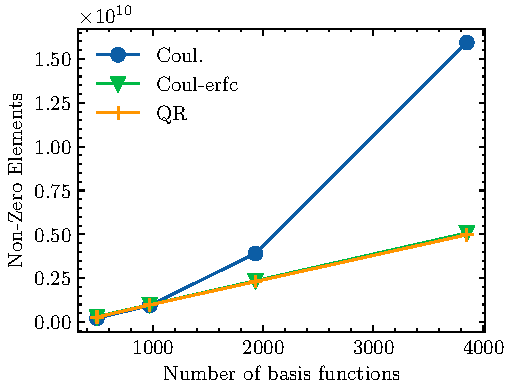
\includegraphics[width=\textwidth]{../articles/art1/ftmp2_nze_alkan}
%\captionof{figure}[This Figure]{Figure}
\end{minipage}
\begin{minipage}{0.4\textwidth}
\begin{tabular}{rrrr}
\hline
N$_{AO}$ & DFCM & DFCAM & QRDF \\ \hline
490 & --- & --- 	& --- \\ 
970	& 2.14 & 1.69 & 1.80 \\
1930	 & 2.06 & 1.26 & 1.25 \\
3850	 & 2.03 & 1.11 & 1.11 \\
 \hline
\end{tabular}
%\captionof{table}[This Table]{REDO THIS!!!!}
\end{minipage}
\caption{Sparsity behaviour of the intermediate tensor $\mbf{D}$ in the Z kernel for the first Laplace point.}
\label{fig:GS_ZMEM_LA}
\end{figure}

\begin{figure}
\begin{minipage}{0.5\textwidth}
\centering
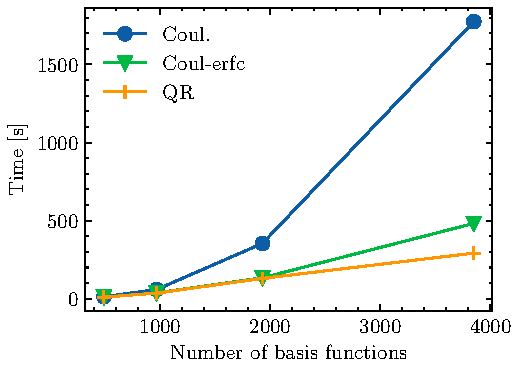
\includegraphics[width=\textwidth]{../articles/art1/mp2_alkan}
%\captionof{figure}[This Figure]{Figure}
\end{minipage}
%\hspace{0.05\textwidth}
\begin{minipage}{0.4\textwidth}
\centering
\begin{tabular}{rrrr}
\hline
N$_{AO}$ & DFCM & DFCAM & QRDF \\ \hline
490 & --- & --- 	& --- \\ 
970	& 2.45 & 1.96 & 2.09 \\
1930	 & 2.55 & 1.82 & 1.83 \\
3850	 & 2.00 & 1.59 & 1.00 \\
 \hline
\end{tabular}
%\captionof{table}[This Table]{REDO THIS!!!!}
\end{minipage}
\caption{Average wall times for the construction of the Z kernel and scaling coefficients (LA)}
\label{fig:GS_ZSCALE_LA}
\end{figure}

\begin{figure}
\begin{minipage}{0.5\textwidth}
\centering
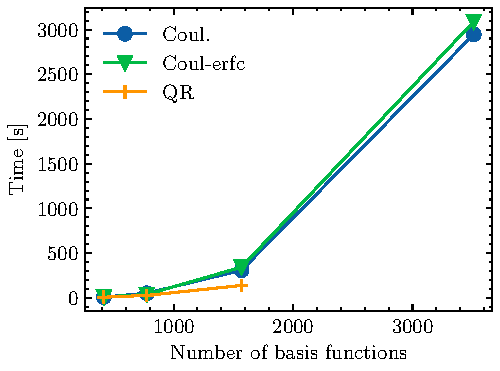
\includegraphics[width=\textwidth]{../articles/art1/mp2_fw}
%\captionof{figure}[This Figure]{Figure}
\end{minipage}
%\hspace{0.05\textwidth}
\begin{minipage}{0.4\textwidth}
\centering
\begin{tabular}{rrrr}
\hline
N$_{AO}$ & DFCM & DFCAM & QRDF \\ 
490 & --- & --- & --- \\ 
970 & 2.51 & 1.88 & 1.88 \\ 
1930 & 2.59 & 3.18 & 2.36 \\ 
3850 & 3.26 & 3.18 & --- \\ 
 \hline
\end{tabular}
%\captionof{table}[This Table]{REDO THIS!!!!}
\end{minipage}
\caption{Average wall times for the construction of the Z kernel and scaling coefficients (FW)}
\label{fig:GS_ZSCALE_FW}
\end{figure}

\begin{table}
\centering
\begin{tabular}{cccc}
 \hline
 & Coul. & Coul-erfc & QR\\ \hline 
alkan20 & 28.81 & 28.76 & 28.85 \\ 
alkan30  & 29.04 & 29.02 & 29.14 \\ 
alkan40 & 28.38 & 28.38 & 28.50 \\ 
FW15 & 23.31 & 23.29 & 23.27 \\ 
FW21 & 23.27 & 23.26 & 23.26 \\ 
FW30 & 24.30 & 24.20 & 24.10 \\ 
\hline 
\end{tabular}
\caption{SOS-MP2 energy differences in $\mu$Hartrees per occupied orbital compared to the canonical SOS-MP2 reference.}
\label{fig:GS_ZACCURACY}
\end{table}

\section{Atomic Orbital ADC}

\subsection{Molecular Test Systems}

For the performance analysis of AO-ADC(2), again two molecular systems are chosen: linear carboxylic acids (LCA, Figure \ref{fig:ACID}) and the hydrated formamide systems (FW) from the previous section. The LCAs were optimized using DFT/B3LYP and the 6-31G* basis set.

Two major factors influence the performance of local excited state methods: locality of electron correlation, and locality of the excitation space. The LCA systems form the best case scenario for both types of locality. The atomic ground state density becomes sparse very rapidly with increasing chain length, and so does the atomic transition density for the lowest lying singlet excitation. The excitation space for that transition is localized on the COOH group, and the number of elements in the transition density matrix scales with with $\mathcal{O}(1)$ in the limit of large systems. On the other hand, FW has a non-sparse AO ground state density, but a sparse AO transition density. Here, the first singlet excited state is localized on the formamide molecule. With increasing size of the solvation shell, the number of significant elements in the transition matrix grows slowly, and the excitation energy will eventually converge to a constant value in the limit of an infinitely large solvation shell \cite{Bau2017}, demonstrating the intensive property of excitations. As such, while FW is a worst case scenario for local ground state calculations, excited state methods are able to exploit the locality of the excitation in order to lower the computational cost.   

\begin{figure}
\centering
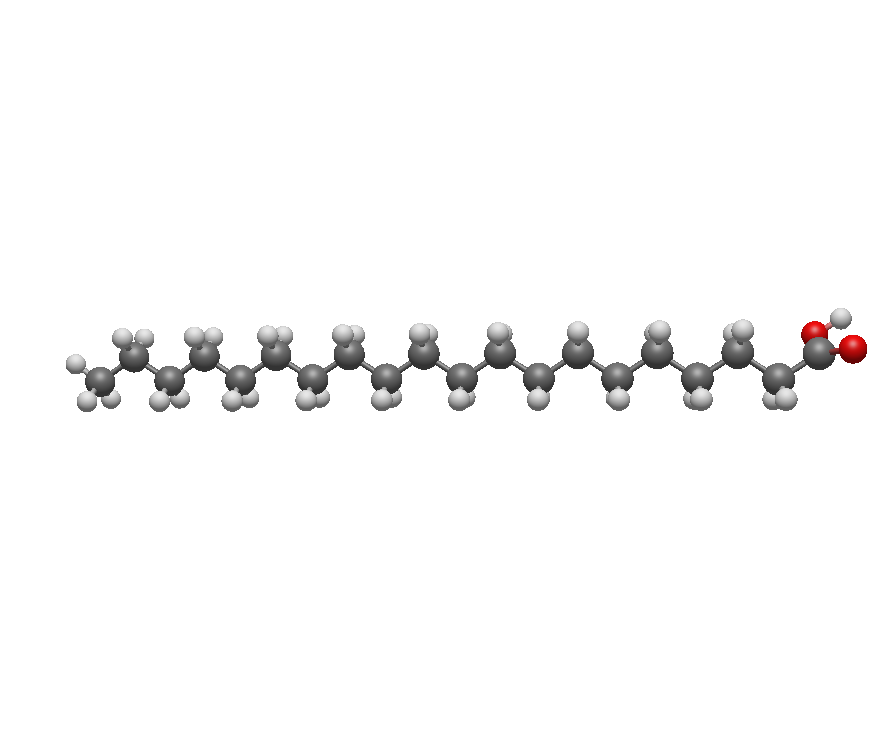
\includegraphics[width=0.5\textwidth]{Pics/acid.png}
\caption{Structure of the linear carboxylic acids (LCA).}
\label{fig:ACID}
\end{figure}

\subsection{Scaling}

For analyzing the scaling of the AO-ADC(2) method, the cc-pVDZ basis set is used, with cc-pVDZ-ri for density fitting. Table \ref{tab:ES_NUMBAS} shows the number of basis functions for the test systems. Furthermore, only the performance of the first matrix-vector product is analyzed, using a (singlet) CIS-optimized transition matrix as the input. The CIS vectors are sparse, and the density of the ADC(2) trial vectors will be of similar sparsity. It should be noted that it is very important to use CIS as the the initial guess, because a guess based on molecular orbital energies can be very dense. 

For evaluating the doubles part of the MVP, the OV version of the algorithm will be used.

Figure \ref{fig:ES_TIME_LCA} shows the performance of the matrix-vector product for the LCA systems. Again, three metrics are used: DFCM, DFCAM ($\omega$ = 0.1) and QRDF ($T$ = 1e-5, $R$ = 40). The atomic orbital formulation of ADC(2) drastically reduces the scaling from $\ccpx{4}$ to $\ccpx{2}$ for standard density fitting. Using local density fitting, the computational effort can be further pushed down to $\ccpx{1.5}$ and $\ccpx{1}$ for DFCAM and QRDF respectively. The cross-over is very early, and sub-quadratic scaling is already reached at LCA40. The performance of AO-ADC(2) is therefore even better than the predicted $\ccpx{2}$ scaling. This discrepancy is due to the sparsity of the AO transition matrix: during the sparsity analysis, $\ccpx{1}$ scaling was assumed, analogous to the ground state density. However, the transition density scales with $\mathcal{O}(1)$ in the asymptotic limit, which leads to sub-quadratic performance.

Figure \ref{fig:ES_TIMESINGLE_LCA} shows the total wall time for each individual component of the MVP calculation. The evaluation of the intermediate matrices (intermeds) and the doubles-part (2E) are the most expensive steps. The computational timings for computing part 2C, 2D and the CIS Fock matrices (jk) are one order of magnitude lower. Part 2A and 2B only involve a single matrix multiplication of the MO transition matrix with the intermediate matrices, and are therefore evaluated very quickly. The Cholesky decompositions also do not considerably influence the total scaling. 

Concerning the memory footprint of AO-ADC(2), the same 3-index tensors that appeared in the evaluation of the Hartree-Fock and SOS-MP2 ground state energy also appear here: $B_{X\mu\nu}$ (the 3c2e integrals or the QRDF fitting coefficients), $C_{X\mu\nu}$ ($M_{XY}B_{Y\mu\nu}$) and $B\pa_{X\uli\ola}$ ($P\pa_{\mu\mu'} B_{X\mu'\nu'} Q\pa_{\nu'\nu}$. Their sparsity was discussed in detail in the previous section. Additionally, the following tensors need to be stored in memory: $C'_{X\mu\nu}$ ($G_{XY}B_{Y\mu\nu}$ in the K kernel during evaluation of the intermediates, see Algorithm 2), and the intermediate Laplace tensors in the Cholesky MO basis ($B\pt_{X\uli\ola}$, $R\pt_{X\uli\ola}$, $D\pt_{X\uli\ola}$), as defined in the previous chapter in Algorithm 6. The tensors will be abbreviated as $C'$, $B_{MO}$, $R_{MO}$ and $D_{MO}$ for this discussion, and $B_{AO}$ is used for $B_{X\mu\nu}$.

\ref{fig:ES_SPARSITY_LCA} shows the block sparsity of those tensors for QRDF, with $B_{AO}$ as reference points. Block sparsity is defined as the number of significant blocks divided by the total number of blocks in the dense tensor. $C'$ and $B_{MO}$ are very dense, with a block sparsity slightly below 10\%. The intermediate Laplace tensors $D_{MO}$ and $R_{MO}$ decay much faster than $B_{AO}$ which was shown to scale with $\ccpx{N}$. For LCA160, $I_{MO}$ and $R_{MO}$ are an order of magnitude sparser ($\approx$ 0.1\%) than $B_{AO}$. The difference to the other Laplace tensor $B_{MO}$ is that $I_{MO}$ and $R_{MO}$ are formed by the contraction of $B_{AO}$ with both the AO ground state density $\mbf{P}$ and the AO transition matrix $\mbf{U}$, which explains their much higher degree of sparsity compared to $B_{MO}$ which is formed using the AO ground state densities only. One peculiar thing to notice here is that the intermediate tensor $D_{MO}$, which is formed from $B_{MO}$ and $R_{MO}$, is sparser than both of its input tensors. This indicates a potentially faster route to evaluating $D_{MO}$ by imposing sparsity criteria on $B_{MO}$ and $R_{MO}$. How these criteria exactly look like is subject of future investigation. The most plausible route goes via a sparsity analysis of the trial vector $u$, similar to how LMO or NO excited state methods generate a compact virtual orbital space.

Similarly, the evaluation of the intermediate tensors can be sped up by only taking into the account the AOs which are near or within the excitation space. This would however lead to a loss of state specificity of the AO-ADC(2) MVP. 

Figure \ref{fig:ES_TIME_FW} shows the performance of AO-ADC(2) for solvated formamide. Although the density of the systems negatively impacts performance compared to LCA, it is still possible to achieve sub-cubic scaling thanks to the sparsity of the AO transition matrix. The point for FW144 with DFCAM is missing due to numerical issues that were encountered during the calculation. Nonetheless, the graph speaks for the success of the AO-ADC(2), even for non-ideal systems, provided that the excitation space is small. Figure \ref{fig:ES_SPARSITY_FW} shows the block sparsity of the tensors discussed in the previous paragraphs for LCA. Although most tensors are very dense, the intermediate $D_{MO}$ almost falls below the 0.1\% mark. Similarly to LCA, this sparsity might be used for imposing conditions on the other tensors, and speeding up the calculations for all components of the AO-ADC(2) vector. 

\begin{table}
\centering
\begin{tabular}{llllll}
\hline
\multicolumn{3}{c}{LCA} & \multicolumn{3}{c}{FW} \\ \hline
Molecule & Abbrev. & $N_{AO}$ & Molecule & Abbrev. & $N_{AO}$ \\ \hline
H$_{41}$C$_{20}$O & LCA20 & 508 & H$_{33}$CNO$_{16}$ & FW15 & 417 \\
H$_{81}$C$_{40}$O & LCA40 & 988 & H$_{63}$CNO$_{31}$ & FW30 & 777 \\
H$_{161}$C$_{80}$O & LCA80 & 1948 & H$_{129}$CNO$_{64}$ & FW63 & 1569 \\
H$_{321}$C$_{160}$O & LCA160 & 3868 & H$_{291}$CNO$_{145}$ & FW144 & 3513 \\
\hline
\end{tabular}
\label{tab:ES_NUMBAS}
\caption{Total number of basis functions for linear carboxlyic acids (LCA) and solvated formamide (FW) with the aug-cc-pVDZ basis set}
\end{table}

\begin{figure}
\begin{minipage}{0.5\textwidth}
\centering
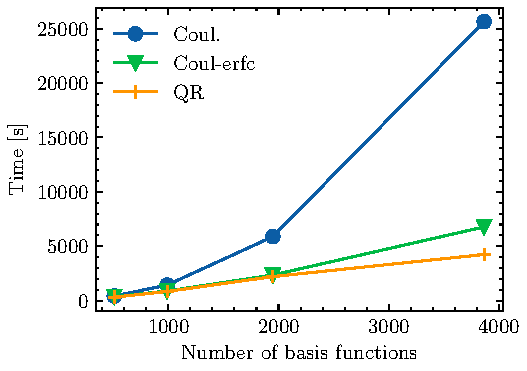
\includegraphics[width=0.9\textwidth]{../articles/art2/adctime_acid}
%\captionof{figure}[This Figure]{Figure}
\end{minipage}
\begin{minipage}{0.4\textwidth}
\centering
\begin{tabular}{rrrr}
\hline
N$_{AO}$ & DFCM & DFCAM & QRDF \\ \hline
508 & --- & --- & --- \\ 
988 & 1.8 & 1.4 & 1.5 \\ 
1948 & 2.1 & 1.5 & 1.4 \\ 
3868 & 2.2 & 1.5 & 1.0 \\
 \hline
\end{tabular}
%\captionof{table}[This Table]{REDO THIS!!!!}
\end{minipage}
\caption{Performance of a single matrix-vector-product with a CIS optimized (singlet) trial vector, for linear carboxylic acids.}
\label{fig:ES_TIME_LCA}
\end{figure}

\begin{figure}
\centering
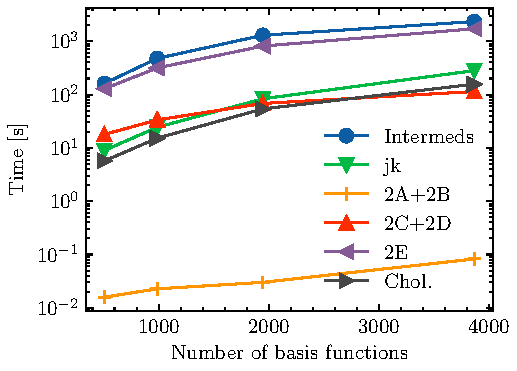
\includegraphics[scale=1.0]{../articles/art2/adcsingle_acid}
\caption{Figure}
\caption{Total time needed to evaluate each separate component of the MVP using quasi-robust density fitting (linear carboxylic acid)}
\label{fig:ES_TIMESINGLE_LCA}
\end{figure}

\begin{figure}
\centering
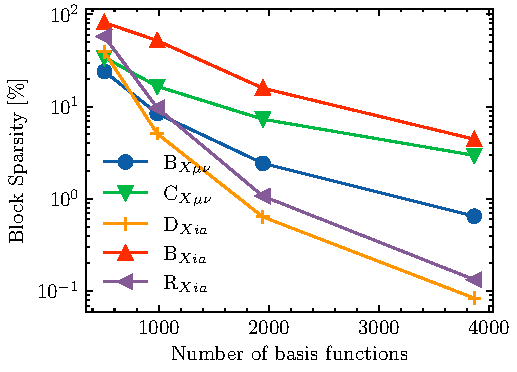
\includegraphics[scale=1.0]{../articles/art2/blocksparsity_acid}
\caption{Block sparsity for the major 3-index tensors appearing in the evaluation of the MVP (linear carboxylic acid)}
\label{fig:ES_SPARSITY_LCA}
\end{figure}

\begin{figure}
\begin{minipage}{0.5\textwidth}
\centering
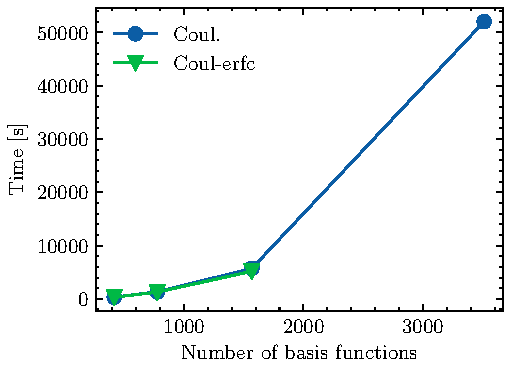
\includegraphics[width=0.9\textwidth]{../articles/art2/adctime_fw}
%\captionof{figure}[This Figure]{Figure}
\end{minipage}
\begin{minipage}{0.4\textwidth}
\centering
\begin{tabular}{rrr}
\hline
N$_{AO}$ & DFCM & DFCAM \\ \hline
508	& ---	& --- \\
988	& 2.3	& 2.3 \\
1948 & 	2.1 &	2.0 \\
3868	 & 2.74 & --- \\
 \hline
\end{tabular}
%\captionof{table}[This Table]{REDO THIS!!!!}
\end{minipage}
\caption{Performance of a single matrix-vector-product with a CIS optimized (singlet) trial vector, for hydrated formamide.}
\label{fig:ES_TIME_FW}
\end{figure}

\begin{figure}
\centering
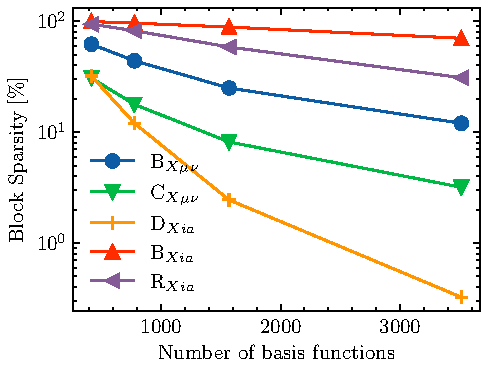
\includegraphics[scale=1.0]{../articles/art2/blocksparsity_fw}
\caption{Block sparsity for the major 3-index tensors appearing in the evaluation of the MVP (hydrated formamide)}
\label{fig:ES_SPARSITY_FW}
\end{figure}

\subsection{Accuracy}

To get an impression on the accuracy that can be achieved with AO-ADC(2), the lowest lying singlet excitation energies for a small set of molecules are compared to the exact results obtained with canonical SOS-ADC(2), as implemented in Q-Chem. The Hartree-Fock wave function is optimized using standard density fitting without any local approximations as the reference for AO-ADC, while the exact HF ground state is used for the canonical calculation. The aug-cc-pVDZ basis set, and the auxiliary basis sets cc-pVTZ-jkfit and aug-cc-pVDZ-ri are used for Hartree-Fock and AO-ADC(2) respectively. The test systems include linear alkanes and carboxylic acids, solvated formamide, as well as the borondipyrromethene-flavin dyad (FLVA) \cite{Kat2007} and the phenothiazine-isoalloxazine dyad (DYAP) \cite{Cra2002}. The structures of FLVA and DYAP are given in Figure \ref{fig:FLVADYAP}.

%  Kats, D.; Korona, T.; Schütz, M. Transition strengths and first-order properties of excited states from local coupled cluster CC2 response theory with density fitting. J. Chem. Phys. 2007, 127, 064107.
% Iso Crawford, T. D.; King, R. A. Locally correlated equation-of-motion coupled cluster theory for the excited states of large molecules. Chem. Phys. Lett. 2002, 366, 611. 

Before considering the results, it is important to note that convergence issues were commonly encountered in the Davdison procedure when using local density approximations. This is due to linear dependencies in the auxiliary basis set space, which then leads to numerical issues in the local density fitting procedure. For DFCAM, the matrix of the 2c2e integrals in the coulomb-attenuated metric, i.e. $\cn{X}{Y}_{\omega}$ needs to be inverted. This can be done by solving the eigenvalue problem, then scaling the eigenvectors by the inverse of the eigenvalues. However, for a linearly dependent basis set, the eigenvalues are very small, which leads to large entries in $\cn{X}{Y}_{\omega}$, and a loss of accuracy. The error propagates through the Davidson iterations and causes convergence issues in the form of negative excitation energies. Fortunately, the problem can often be solved by filtering out all eigenvectors with an associated eigenvalue below a certain threshold (typically around 1e-6 to 1e-4). In the quantum chemistry community, this procedure is known as \emph{canonical orthogonalization}, and gives an approximation to the exact matrix inverse. Alternatively, the problem can be solved by removing the linear dependencies from the basis set itself (see Annex \ref{sec:LINDEP}). Finally, a less diffuse basis set can be used as well. For example, instead of using aug-cc-pVDZ-ri, one may use cc-pVTZ-ri.

However, none of these methods worked for the "strict" QRDF. Due to the harsh screening procedure for the test functions mentioned in the previous sections, many matrix entries of the rectangular matrix $\cn{Q_{test}}{P_{fit}}$ will be very small. This leads to numerical issues when solving the linear-least squares problem, even with linear dependencies removed. Here, an alternative QRDF algorithm is used (see \ref{sec:IMPL_QRDF}), where the test functions are chosen by a weighted average criteria using the auxiliary overlap matrix, with the parameters $T$ = 1e-4 and $S$ = 1e-4. Numerical issues can be completely avoided, as a QR decomposition is more robust than matrix inversion. (TO DO: SHOW SCALING)

Table \ref{tab:ES_ACCURACY} shows the SOS-ADC(2) excitation energy differences in $\mu$Hartrees per occupied orbital. Values are given for DFCM, DFCAM with attenuation factors 0.1 and 1.0, and the improved QRDF algorithm. DFCM shows acceptable accuracy, on the order of several $\mu$Hartrees for the linear systems LCA12, LCA20 and LA20. The errors are even lower for the other test systems. As expected, DFCAM introduces much larger errors, similar to Hartree-Fock. The iterative nature of the Davidson procedure therefore has a significant impact on accuracy for DFCAM. The largest errors are again observed for linear molecules, especially for DFCAM(1.0) where errors for LA20 are almost two orders of magnitude larger. Errors are much smaller for QRDF, and even problematic systems like LA20 have similar accuracy to DFCM, again showing the superiority of the quasi-robust density fitting scheme. Only a single set of parameters for QRDF was used for testing accuracy. A more extensive benchmark, as well as the impact of diffuse basis sets on scaling, are subjects for further investigation.

%It is recommended to use DFCAM(0.1) for a good mix between accuracy and performance, while the QRDF method is unavailable. Furthermore, diffuse auxiliary basis sets should be avoided and substituted for the next highest zeta-level basis set ($D \rightarrow T$, $T \rightarrow Q$, ...). QRDF is expected to perform much better than DFCAM, with similar accuracy to DFCM.

\begin{table}
\centering
\begin{tabular}{lllll}
\hline
System & Coul. & Coul-erfc (0.1) & Coul-erfc (1.0) & QRDF (new) \\
\hline
LCA12	& 3.48	& 0.11	& 2.02	& 2.70 \\
LCA20	& 1.52	& 4.01	& 22.66	& 1.32 \\
LA20	 & 0.90	& 6.29	& 1.24	& 0.50 \\
FW10	 & 0.09	& 6.37	& 0.70	& 0.20 \\
FW15	 & 0.49	& 0.62	& 0.86	& 0.10 \\
FLVA	 & 0.26	& 0.04$^{(a)}$	& 5.25$^{(a)}$	& 0.26 \\
DYAP	 & 1.77	& 27.25	& 94.89	& 1.76 \\
\hline
\end{tabular}
\label{tab:ES_ACCURACY}
\caption{Difference in excitation energy between canonical SOS-ADC(2) and CD-DF-SOS-ADC(2), in $\mu$Hartrees per occupied orbital, for different density fitting approximations. LA = linear alkane, LCA = linear carboxylic acid, FW = solvated formamide, flva(a) = borondipyrromethene-flavin dyad, iso = phenothiazine-isoalloxazine dyad. $^{(a)}$ The cc-pVTZ-ri auxiliary basis set was used instead of aug-cc-pVDZ-ri due to convergence problems.}
\end{table}

\begin{figure}
\centering
\begin{minipage}{0.45\textwidth}
\centering
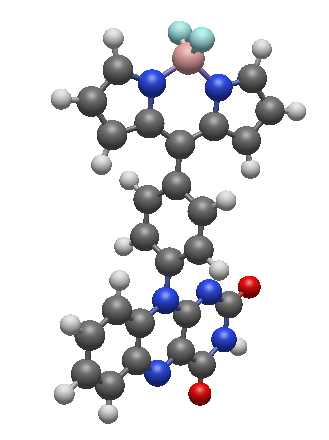
\includegraphics[width=0.9\textwidth]{Pics/FLVA.png}
%\captionof{figure}[This Figure]{Figure}
\end{minipage}
%\hspace{0.05\textwidth}
\begin{minipage}{0.45\textwidth}
\centering
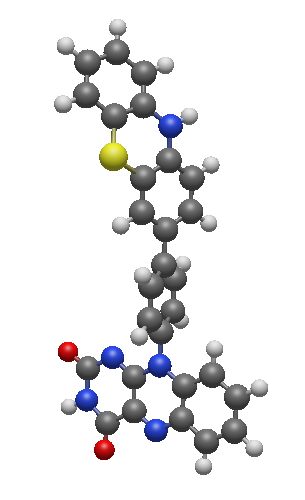
\includegraphics[width=0.9\textwidth]{Pics/DYAP.png}
%\captionof{figure}[This Figure]{Figure}
\end{minipage}
\caption{Molecular structure of borondipyrromethene-flavin (a) and phenothiazine-isoalloxazine (b)}
\label{fig:ES_ACCMOL}
\end{figure}

\subsection{Large Molecules: Challenges and Limitations}

An attempt was made to apply CD-DF-SOS-ADC(2) to chemically interesting molecules with 10,000 basis functions or more, with limited success: even if the atomic orbital formulation can exploit sparsity to reduce the memory footprint and scaling, the need for diffuse basis functions  practically nullifies any advantages it provides. The block occupation with aug-cc-pVDZ or def2-SVPD is still above 50\% for non-linear molecules with $\approx$ 300 atoms, and the very large auxiliary basis sets often lead to OOM (out-of-memory) errors due to data duplication in the QRDF algorithm and other routines. For diffuse auxiliary functions, processes often need to hold the whole $\cn{X}{Y}$ matrix in memory while solving the linear least squares problem. For multiple ranks on a single node, this can quickly lead to memory problems. While memory duplication can be reduced by simply using fewer ranks per node, it should be noted that currently the DBCSR tensor library is only optimized for one MPI rank per CPU. Furthermore, each rank can only allocate approximately 2GB of memory at once, because only 4-byte integers (with maximum value 2,147,483,648) are used to specify the size of the memory window that is allocated. Moreover, the need to reorder the tensors before each contraction effectively doubles the space needed by each tensor (see also the discussion in section \ref{sec:tenstor}).

In ground state methods, OOM errors can often be solved by using \emph{direct} methods where tensors are recomputed on-the-fly. By increasing the number of batches, the memory footprint can be lowered quite considerably. A direct version of CD-DF-SOS-ADC(2) could also be considered, although the need to recompute tensors like $C_{X\mu\nu}$, $R_{X\uli\olgn}$ or $B_{X\uli\olgn}$ multiple times would lead to a much higher prefactor which further pushes the low-scaling regime to larger molecular sizes.

\section{Summary and Outlook}

An atomic orbital formulation of the spin-opposite-scaled algebraic diagrammatic construction method can drastically reduce the formal quartic scaling of canonical, density-fitted SOS-ADC(2). This method, named CD-DF-SOS-ADC(2), can successfully exploit the sparsity of the AO ground state density and the AO transition density. Furthermore, local density fitting significantly reduces the overhead, and the low scaling regime is more easily reached. For linear carboxylic acids, the method scales linearly, and even electron-dense systems, like hydrated formamide, were shown to have sub-cubic scaling if the transition density is sparse. The 3-index tensors necessary for an AO-ADC(2) calculation show a high degree of sparsity, which, when using block-sparse matrix storage, significantly reduces the memory footprint. Furthermore, the high prefactor of AO-ADC(2) can be mitigated using local density fitting, making it somewhat competitive with canonical density-fitted SOS-ADC(2) for less sparse systems, although with a larger memory footprint.

Accuracy was shown to be within acceptable range for standard density fitting and quasi-robust density fitting. Convergence issues were encountered due to linear dependencies with the auxiliary basis sets, which can be addressed by removing certain basis functions, by canonical orthogonalization of the metric inverse, or by just using another basis set. 

Unfortunately, the need for augmented basis sets negatively impacts the scaling of CD-DF-SOS-ADC(2) and delays the onset of the linear-scaling regime. Compared to NO methods, CD-DF-SOS-ADC(2) includes all atomic orbitals and molecular orbitals, as opposed to only the ones close to the excitation region, making it more computationally expensive, although it has the advantage of not being state-specific. 

Pushing the current implementation of CD-DF-SOS-ADC(2) to system sizes with a large number of basis functions ($>$ 5000 basis functions) quickly leads to memory problems, even on distributed systems. This, in combination with diffuse basis functions and molecular systems that are not strictly linear in nature, as well as the increased algebraic complexity of the working equations, means that CD-DF-SOS-ADC(2) cannot really reach the low-scaling regime except in very specific cases. Introducing similar pre-screening techniques to NO methods based on some CIS or CIS(D) density might be beneficial. Moreover, a less memory-intensive tensor library should also be considered. However, at the moment, there are no other tensor libraries besides DBCSR that are well suited. Further development of sparse block tensor libraries are crucial for the future of atomic orbital based methods.

The equations for computing triplet excitations have not yet been implemented, but similar scaling and accuracy to singlet excitations are expected. 